\question[10] \textbf{Determina el volumen del cilindro de la figura \ref{fig:vol_cil_08}.}\\
\textit{Ingresa una respuesta exacta en términos de $\pi$, o usa 3.14.}

\begin{minipage}{0.3\linewidth}
    \begin{figure}[H]
        \begin{center}
            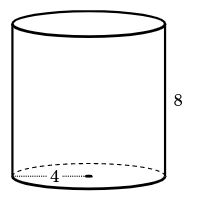
\includegraphics[width=0.75\textwidth]{../images/vol_cil_08.png}
        \end{center}
        \caption{}
        \label{fig:vol_cil_08}
    \end{figure}
\end{minipage}
\begin{minipage}{0.7\linewidth}
    \begin{solutionbox}{6cm}        El volumen de un cilindro de radio $r$ y altura $h$ es:
        \begin{equation*}
            V = \pi r^2 h
        \end{equation*}
        De la figura \ref{fig:vol_cil_08} se sabe que $r=2$ y $h=5$, entonces
        \begin{equation*}
            \begin{split}
                V & = \pi r^2 h\\
                & = \pi (4)^2 (8)\\
                & = \pi (16) (8)\\
                & = 128\pi
            \end{split}
        \end{equation*}
    \end{solutionbox}
\end{minipage}